%auto-ignore
\documentclass[tikz]{standalone}

\usetikzlibrary{calc}

\begin{document}
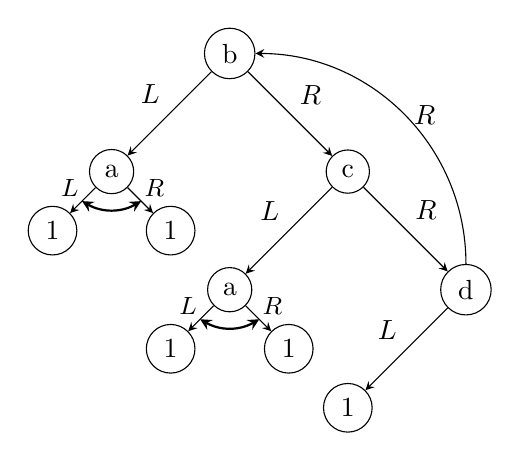
\begin{tikzpicture}[scale=1.5,>=stealth]

\node [circle,draw=black] (n0) at ( 0,  0) {b};
\node [circle,draw=black] (n1) at ( 1, -1) {c};
\node [circle,draw=black] (n2) at ( 2, -2) {d};

\node [circle,draw=black] (m1) at (-1, -1) {a};
\node [circle,draw=black] (m2) at ( 0, -2) {a};
\node [circle,draw=black] (m3) at ( 1, -3) {1};


\node [circle,draw=black] (m11) at (-1-0.5, -1-0.5) {1};
\node [circle,draw=black] (m12) at (-1+0.5, -1-0.5) {1};
\draw [<->,thick] ($(m1)!0.5!(m11)$) to [bend right] ($(m1)!0.5!(m12)$);
\draw [->] (m1) to node [above left=-0.2em] {\small$L$} (m11);
\draw [->] (m1) to node [above right=-0.2em] {\small$R$} (m12);

\node [circle,draw=black] (m21) at ($(m2)+(-0.5,-0.5)$) {1};
\node [circle,draw=black] (m22) at ($(m2)+( 0.5,-0.5)$) {1};
\draw [<->,thick] ($(m2)!0.5!(m21)$) to [bend right] ($(m2)!0.5!(m22)$);
\draw [->] (m2) to node [above left=-0.2em] {\small$L$} (m21);
\draw [->] (m2) to node [above right=-0.2em] {\small$R$} (m22);




\path[->]
	(n0) edge node [above right] {$R$} (n1)
	edge node [above left] {$L$} (m1)
	(n1) edge node [above right] {$R$} (n2)
	edge node [above left] {$L$} (m2)
	(n2)
		edge node [above left] {$L$} (m3)
		edge [bend right=45] node [right] {$R$} (n0)
;

\end{tikzpicture}
\end{document}